\chapter{Introduction}
	The experimental and theoretical study of graphene is a very rapid growing field in modern physics (\ref{fig:grapheneManuscripts}), which is mainly because of the physical milestones of Andre Geim and Konstantin Novoselov. They discovered the first true 2D crystal ever observed in nature : \textbf{graphene}. Both got credited from the Royal Swedish Academy of Science with the Nobel Prize in Physics (2010). The existence of graphene-like materials has often been doubted due to the \textit{Mermin-Wagner theroem}, which states that a 2D crystal melts at any small but non zero temperature. Graphene has the thickness of only one atom and is nevertheless stable, though many believed it was impossible for such a thin crystalline material to be stable. Furthermore graphene, which is based on carbon has some very powerful properties. It is the thinnest, but also strongest known material with the best heat conductivity. It is transparent, conducts electricity as good as copper and is yet so dense, that not even Helium can pass it. The electrons in graphene show relativistic behavior and thus it can be an ideal candidate for proving theoretical quantum-field models. Moreover graphene can be used as transistors faster by far than common silicon ones. In addition its properties of transparency and conductivity combined with the enormous stability and thickness make it a perfect material for new touch screens, light panels or even solar cells. \\
	\begin{figure}[H]
		\centering
		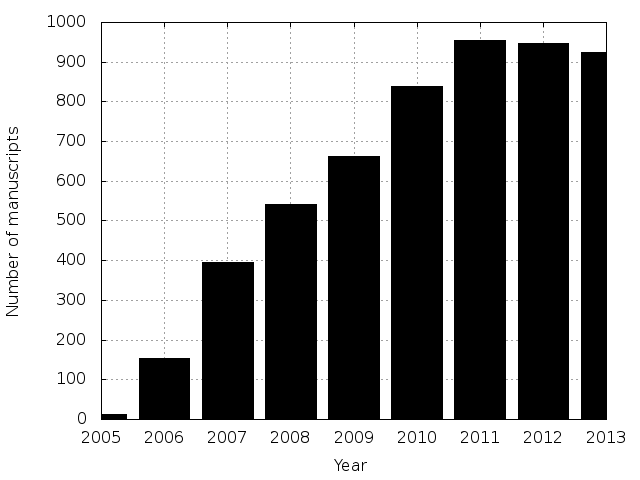
\includegraphics[width=0.7\textwidth]{figures/Introduction/grapheneManuscripts.png}
		\caption{Number of manuscripts with the title 'graphene' posted on www.arxiv.org from the years 2005 to 2013. As one can see, there is an exponential growth from 2005-2008 and a climax right after awarding the nobel prize in 2010.}
		\label{fig:grapheneManuscripts}
	\end{figure}
	\begin{figure}[h]
		\centering
		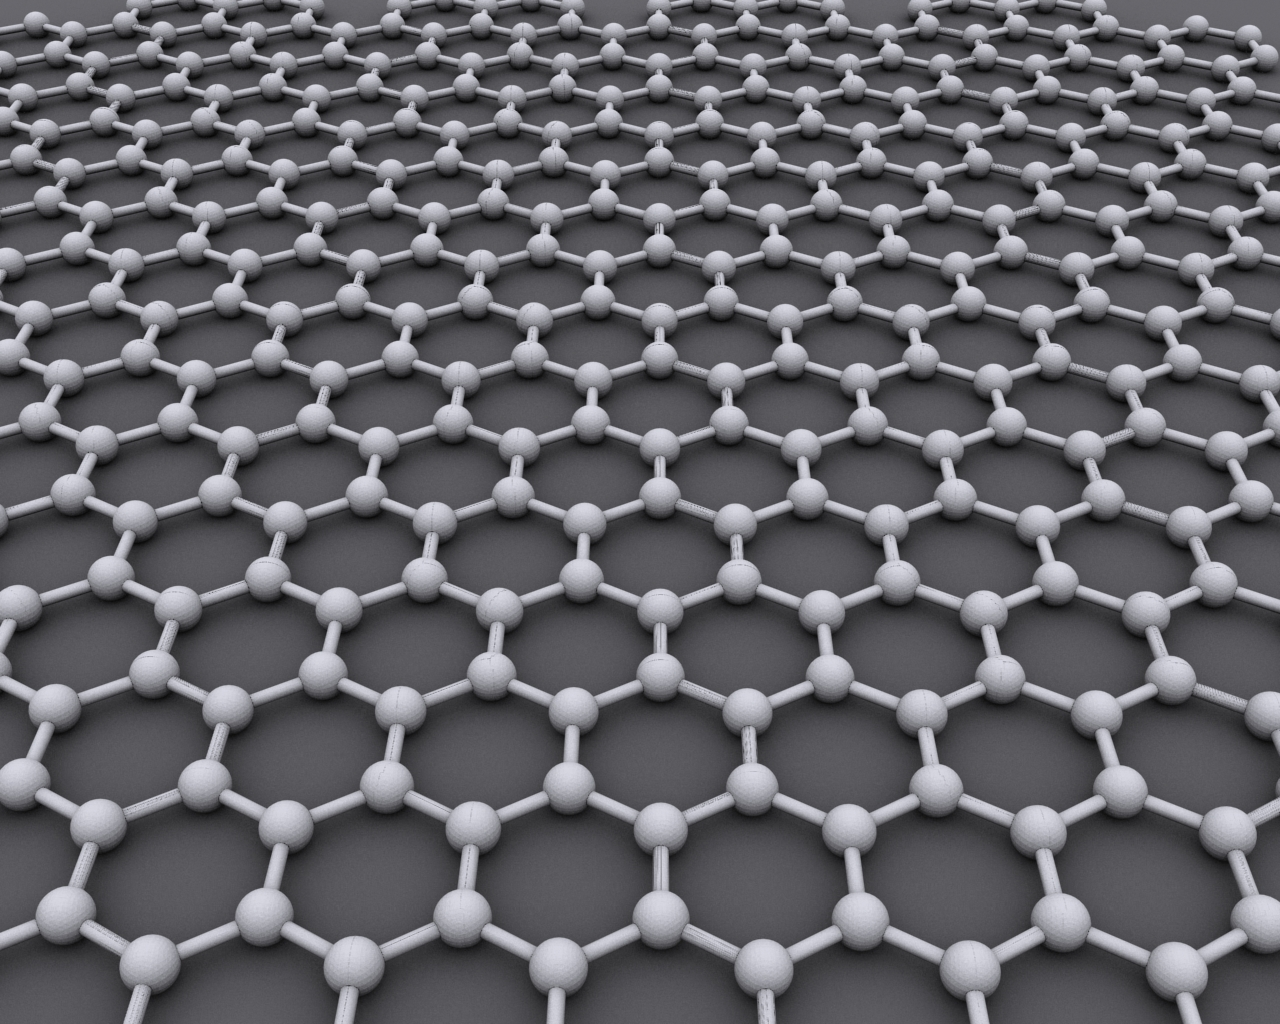
\includegraphics[width=0.7\textwidth]{figures/Introduction/Graphen.jpg}
		\caption{Graphene lattice. Figure taken from \cite{deWikiGraphen}. }
	\end{figure}	
	\noindent As the manufacturing of graphene is a complicated process one can never exclude impurities. In the following chapters we will discuss the effect of some basic impurities in a graphene lattice. We will start with an introduction to solid state physics and continue with some details about carbon materials. Later on we will discuss the calculations made from the density functional theory and the tight binding model.